\chapter{Diffraction by semi-infinite breakwater (break)}

\section{Purpose}

This case models wave diffraction occurring at the point of a semi-infinite
breakwater \cite{Penney1952}.
This process is extremely important as tsunami waves travel a long way and
is subject to diffraction around islands, headlands etc., and is subject to
refraction wherever there are significant variations of water depth.

\section{Description}

This case is the analytical solution for a sinusoidal train of waves travelling
north and diffracting around the tip of a semi-infinite breakwater along the
positive $x$-axis as depicted in Figure \ref{t2d:break:fig:AnalSol}.

\begin{figure}[!htbp]
 \centering
 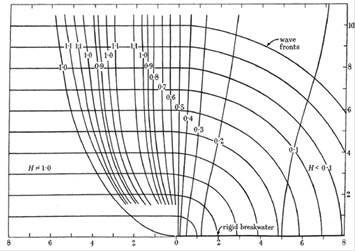
\includegraphics[width=0.4\textwidth]{img/AnalyticSolutionBreak.png}
 \caption{Wave fronts and contour lines of maximum wave heights in the lee of a breakwater. Waves are coming from the south.}
 \label{t2d:break:fig:AnalSol}
\end{figure}

The water depth is taken uniform so that the wave celerity is constant everywhere.
The water depth is also taken sufficiently low that the wave length is greater
than 20 times the water depth and so the shallow water wave equations are valid.
The wave amplitude is also taken very small so as to minimise nonlinear effects.

\subsection{Numerical and physical parameters}
The \telemac{2D} flow model is run using the wave equation formulation and no
friction or viscosity.
The implicitation coefficients are taken as 0.501 (the model is second order
accurate if implicitation = 0.5, but on the edge of instability as the scheme is
unstable if implicitation < 0.5) and the free surface gradient compatibility is
taken as 0.9 (recommended value).

\subsection{Boundary conditions}
The incident wave boundary condition (from the south) is taken as an absorbing
wave paddle and the open exit boundaries (east, west and north) are all taken
as absorbing boundaries using the Thompson boundary condition.
The model extends south of the breakwater so that the tip of the breakwater is
an internal point of the model grid and the boundary condition on the front and
back face of the breakwater is a solid wall (100~\% reflection condition).

Figure \ref{t2d:break:fig:BC} shows the types of boundary conditions.
\begin{figure}[!htbp]
 \centering
 \includegraphicsmaybe{[width=0.9\textwidth]}{../img/BC.png}
 \caption{Boundary conditions types.}
 \label{t2d:break:fig:BC}
\end{figure}

\section{Results}
In Figure \ref{t2d:break:fig:AnalSol} the $y$ axis shows distance from the
breakwater line non-dimensionalised by the wave length.
Figure \ref{t2d:break:fig:WaveAmplitude} shows a comparison between the wave
amplitude from the model and the analytical solution along two lines parallel to
and behind the breakwater at two and eight wavelengths.

\begin{figure}[!htbp]
 \centering
 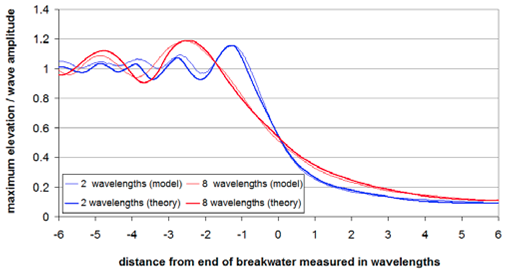
\includegraphics[width=0.5\textwidth]{img/WaveAmplitude.png}
 \caption{Wave amplitude along two lines parallel to and behind the breakwater at 2 and 8 wavelengths. Model (thin lines) and analytical (thick lines) solutions.}
 \label{t2d:break:fig:WaveAmplitude}
\end{figure}


Free surface elevation and velocity magnitude at the end of the simulation
can be seen in Figures \ref{fig:break:FreeSurface} and
\ref{fig:break:Velocity}.

\begin{figure}[H]
 \centering
 \includegraphicsmaybe{[width=0.9\textwidth]}{../img/FreeSurface.png}
 \caption{Free surface elevation at final time.}
 \label{fig:break:FreeSurface}
\end{figure}

\begin{figure}[H]
 \centering
 \includegraphicsmaybe{[width=0.9\textwidth]}{../img/Velocity.png}
 \caption{Velocity magnitude at final time.}
 \label{fig:break:Velocity}
\end{figure}

\section{Conclusion}

The model gives a good representation of the reduction of the wave amplitude in
the lee of the breakwater at two and eight wavelengths from the structure showing
the diffraction process.
The variation of the wave amplitude not in the lee is reasonable but rather less
accurate.
